\documentclass[border=4pt]{standalone}
\usepackage{tikz}
\usetikzlibrary{arrows}
\begin{document}
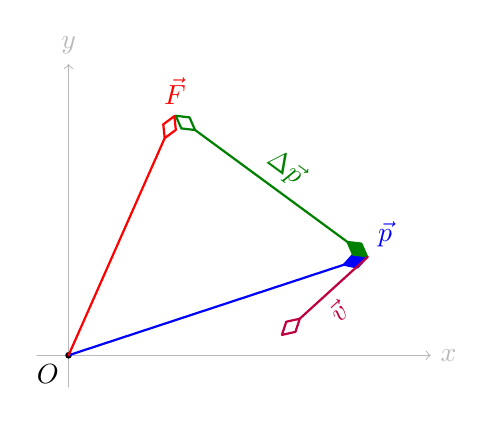
\begin{tikzpicture}[line cap=round]
  \draw[gray!55,->] (-.4,0) -- (4.6,0) node[right] {$x$};
  \draw[gray!55,->] (0,-.4) -- (0,3.7) node[above] {$y$};
  \fill (0,0) circle (1.2pt) node[below left] {$O$};

  \draw[blue,line width=.8pt,-diamond] (0,0) -- (3.8,1.25)
    node[above right] {$\vec p$};
  \draw[red,line width=.8pt,-{open diamond}] (0,0) -- (1.35,3.05)
    node[above] {$\vec F$};
  \draw[green!50!black,line width=.8pt,{diamond}-{open diamond}] (3.8,1.25) -- (1.35,3.05)
    node[midway,above,sloped] {$\Delta\vec p$};
  \draw[purple,line width=.8pt,{open diamond}-] (2.7,.25) -- (3.8,1.25)
    node[midway,below,sloped] {$\vec v$};
\end{tikzpicture}
\end{document}
